%%% -*- TeX-master: "../main" -*-
\chapter{Results}
\label{cha:results}

% TODO: Discussion of why frame reconstruction did not work?

\begin{figure}[h]
  \begin{subfigure}{3in}
  \centering
    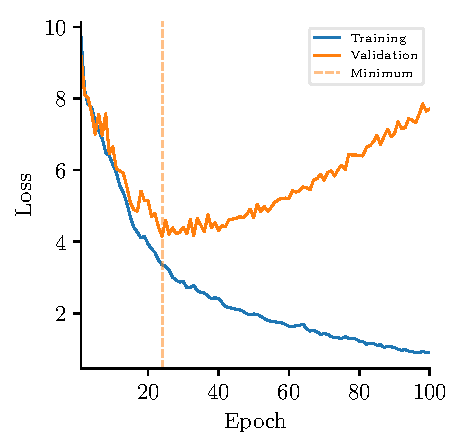
\includegraphics[width=3in]{figures/results/losses/gru-gists}
    \caption{Cross Entropy}
  \end{subfigure}
  \hfill
  \begin{subfigure}{3in}
  \centering
    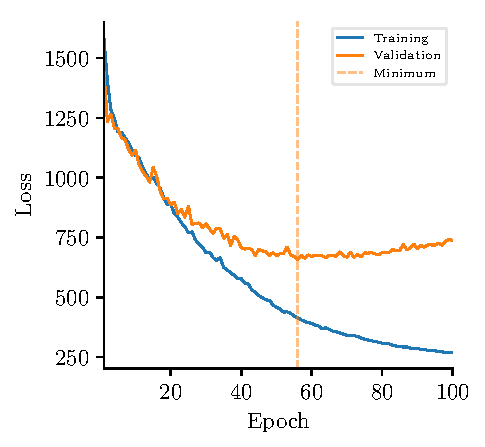
\includegraphics[width=3in]{figures/results/losses/ctc-gists}
    \caption{CTC}
  \end{subfigure}
  \caption{}
  \label{fig:loss-gists}
\end{figure}

\begin{figure}[h]
  \begin{subfigure}{3in}
  \centering
    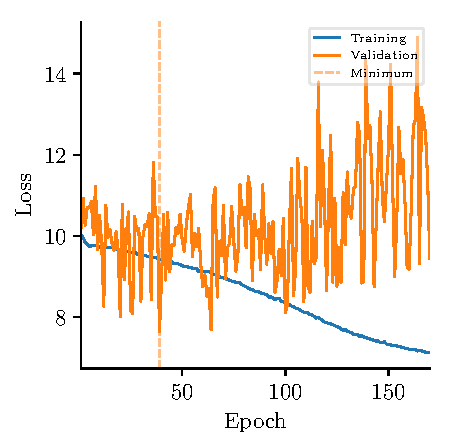
\includegraphics[width=3in]{figures/results/losses/gru-inceptionv3}
    \caption{Cross Entropy}
  \end{subfigure}
  \hfill
  \begin{subfigure}{3in}
  \centering
    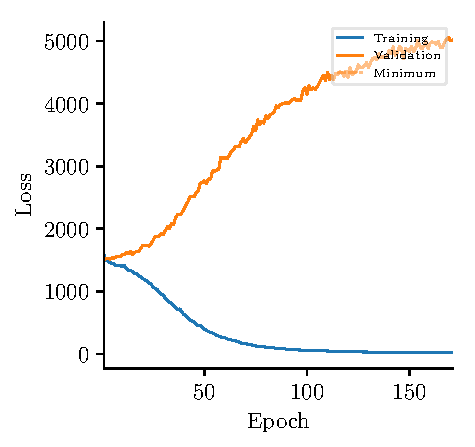
\includegraphics[width=3in]{figures/results/losses/ctc-inceptionv3}
    \caption{CTC}
  \end{subfigure}
  \caption{}
  \label{fig:loss-inceptionv3}
\end{figure}

\begin{figure}[h]
  \begin{subfigure}{3in}
  \centering
    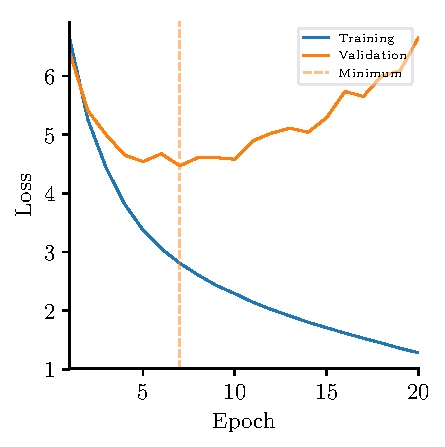
\includegraphics[width=3in]{figures/results/losses/gru-events}
    \caption{Cross Entropy}
  \end{subfigure}
  \hfill
  \begin{subfigure}{3in}
  \centering
    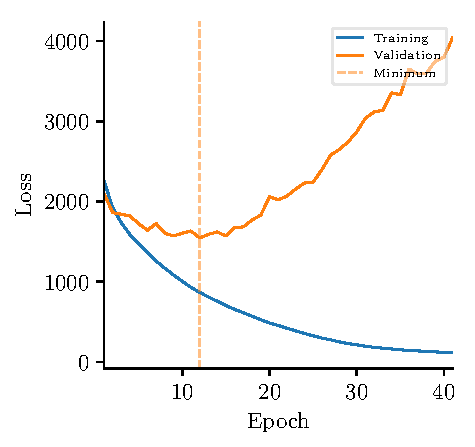
\includegraphics[width=3in]{figures/results/losses/ctc-events}
    \caption{CTC}
  \end{subfigure}
  \caption{}
  \label{fig:loss-events}
\end{figure}

\begin{figure}[h]
  \centering
  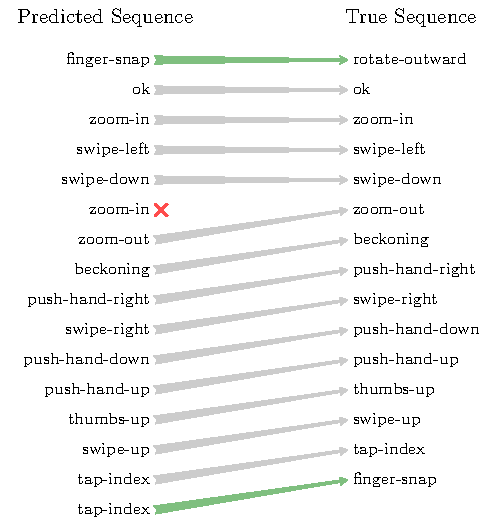
\includegraphics{figures/results/levenshtein}
  \caption{Levenshtein distance of 3}
  \label{fig:levenshtein}
\end{figure}

\begin{table}
  \centering
  \begin{subtable}{\textwidth}
    \centering
    \begin{tabular}{r|c|c|c}
      % BEGIN RECEIVE ORGTBL levenshtein
Method & Events & Gists & InceptionV3\\
\hline
CE + HMM Segmentation & 6.5 & \textbf{2.0} & 14.5\\
CTC + HMM Segmentation & 16.0 & 12.5 & 15.25\\
CE + HMM Decoding & 2104.0 & 22.0 & 16.0\\
CTC + HMM Decoding & 3378.25 & 21.0 & 16.0\\
      % END RECEIVE ORGTBL levenshtein
    \end{tabular}
    \caption{Mean Levenshtein Distance (lower is better)}
  \end{subtable}
  \par\bigskip
  \begin{subtable}{\textwidth}
    \centering
    \begin{tabular}{r|c|c|c}
      % BEGIN RECEIVE ORGTBL label-error-rate
Method & Events & Gists & InceptionV3\\
\hline
CE + HMM Segmentation & 0.406 & \textbf{0.125} & 0.906\\
CTC + HMM Segmentation & 1.0 & 0.781 & 0.953\\
CE + HMM Decoding & 131.5 & 1.375 & 1.0\\
CTC + HMM Decoding & 211.14 & 1.313 & 1.0\\
      % END RECEIVE ORGTBL label-error-rate
    \end{tabular}
    \caption{Label Error Rate (lower is better)}
  \end{subtable}
  \caption{}
  \label{tab:}
\end{table}
\begin{comment}
  #+ORGTBL: SEND levenshtein orgtbl-to-latex :splice t
  | Method                 |  Events |        Gists | InceptionV3 |
  |------------------------+---------+--------------+-------------|
  | CE + HMM Segmentation  |     6.5 | \textbf{2.0} |        14.5 |
  | CTC + HMM Segmentation |    16.0 |         12.5 |       15.25 |
  | CE + HMM Decoding      |  2104.0 |         22.0 |        16.0 |
  | CTC + HMM Decoding     | 3378.25 |         21.0 |        16.0 |
\end{comment}
\begin{comment}
  #+ORGTBL: SEND label-error-rate orgtbl-to-latex :splice t
  | Method                 | Events |          Gists | InceptionV3 |
  |------------------------+--------+----------------+-------------|
  | CE + HMM Segmentation  |  0.406 | \textbf{0.125} |       0.906 |
  | CTC + HMM Segmentation |    1.0 |          0.781 |       0.953 |
  | CE + HMM Decoding      |  131.5 |          1.375 |         1.0 |
  | CTC + HMM Decoding     | 211.14 |          1.313 |         1.0 |
\end{comment}
